\section{Per-vertebral-level results}
\label{app:perlevel}

Table~\ref{tab:perlevel} gives the numeric values behind
Figure~\ref{fig:perlevel}. Chance is the order statistic for that level's
expected-organ set size, so it varies by level; a level ``beats chance'' when its
observed mean rank is strictly below its own chance value.

\begin{table}[H]
\centering
\caption{Per-vertebral-level mean rank against chance, post-correction. $n$ is
the number of rankable lesions at that level (178 of 180 total).}
\label{tab:perlevel}
\begin{tabular}{lrrrl}
\toprule
Level & $n$ & Mean rank & Chance & Verdict \\
\midrule
T1  &  7 & 1.43 & 4.00 & beats chance \\
T2  & 10 & 1.40 & 4.00 & beats chance \\
T3  &  7 & 1.71 & 4.00 & beats chance \\
T4  & 10 & 1.30 & 3.00 & beats chance \\
T5  &  9 & 1.11 & 3.00 & beats chance \\
T6  &  7 & 1.14 & 3.00 & beats chance \\
T7  &  9 & 1.11 & 3.00 & beats chance \\
T8  & 10 & 1.00 & 3.00 & beats chance (perfect) \\
T9  &  7 & 1.00 & 2.00 & beats chance (perfect) \\
T10 & 10 & 1.20 & 2.40 & beats chance \\
T11 & 12 & 1.50 & 2.00 & beats chance \\
T12 & 10 & 1.60 & 1.50 & at/below chance \\
L1  & 17 & 2.41 & 2.00 & at/below chance \\
L2  & 10 & 3.90 & 3.00 & at/below chance \\
L3  & 17 & 2.35 & 4.00 & beats chance \\
L4  & 13 & 1.31 & 3.00 & beats chance \\
L5  & 13 & 3.08 & 3.00 & at/below chance \\
\bottomrule
\end{tabular}
\end{table}

\section{All organ maps on a Spine-Mets slice}
\label{app:organgrid}

The index is computed from the 11 organ maps that Figure~\ref{fig:organgrid}
shows in full. It is reproduced here rather than in the body because eleven
columns cannot be read at single-column width, and because
\S\ref{sec:results:lesion} makes the argument it supports on the two cases in
Figure~\ref{fig:qualitative}, where the distinction between a correct detection
and a phantom is visible.

\begin{figure}[p]
\centering
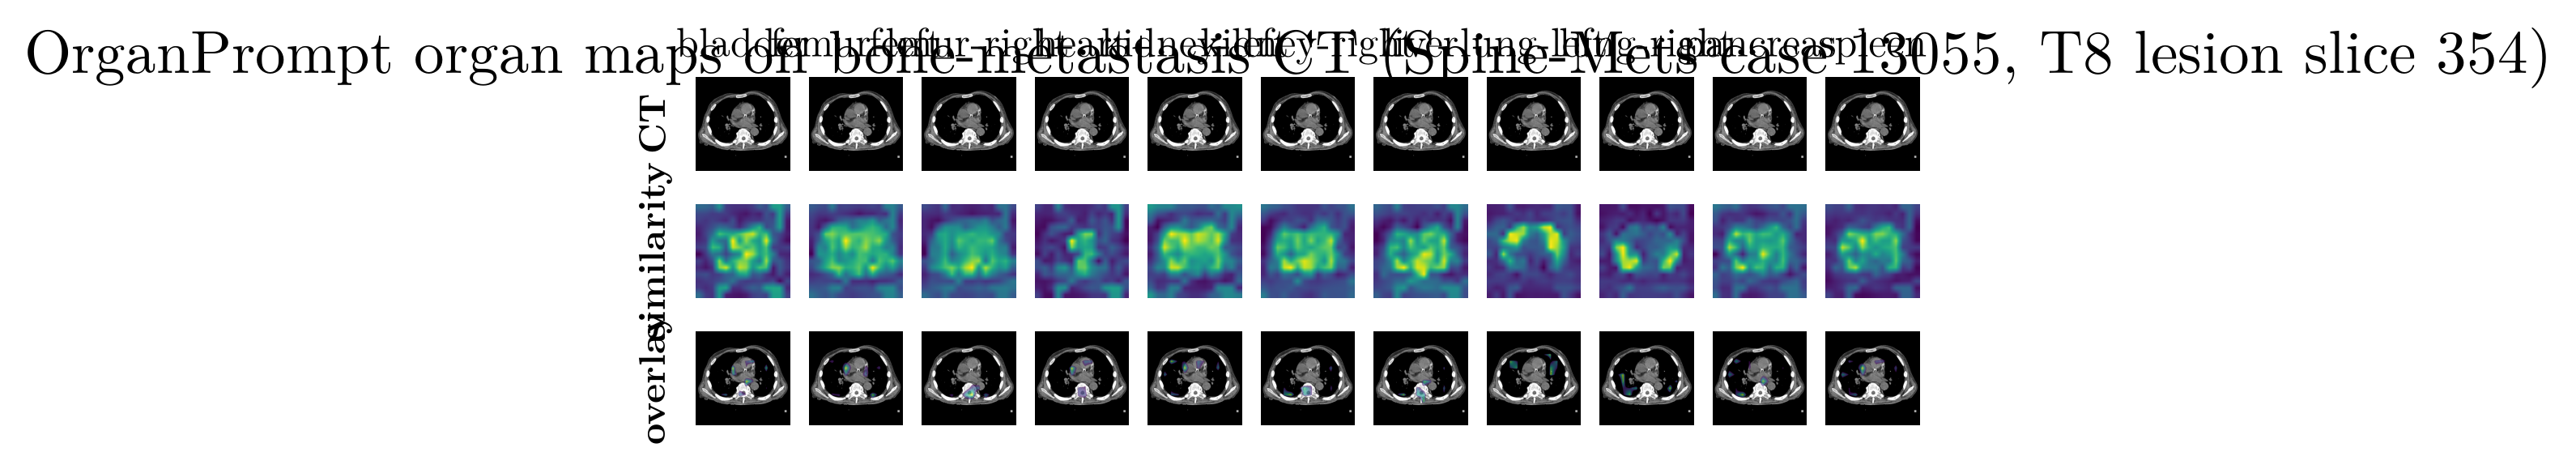
\includegraphics[width=\textwidth]{fig4_spine_organ_grid.png}
\caption{All 11 organ maps on a single Spine-Mets thoracic lesion slice (case
13055, T8 lesion). The rows are the CT slice, the raw patch-text similarity, and
the overlay. The highlight marks the top 2\% of each slice's own similarity
distribution rather than an absolute
cutoff, because raw similarity is routinely negative across an entire slice and
organs win relatively rather than absolutely, so an absolute-zero threshold
renders most panels blank. The panel is the T8 \emph{lesion} slice rather than
the patient's peak-tumor slice, which sits at the pelvis where heart, lungs,
liver and spleen are out of frame; that slice would display noise in those
columns and wrongly imply the model hallucinates organs that are in fact
absent.}
\label{fig:organgrid}
\end{figure}

